\documentclass[12pt,a4paper]{article}

\usepackage[utf8]{inputenc}
\usepackage[T1]{fontenc}
\usepackage[spanish,es-nodecimaldot]{babel}
\usepackage{lmodern}
\usepackage{textcomp}
\usepackage{amsmath,amssymb}
\usepackage{booktabs}
\usepackage{array}
\usepackage{float}
\usepackage{xcolor}
\usepackage{microtype}
\usepackage{tikz}
\usepackage[hidelinks]{hyperref}
\usepackage[a4paper,margin=2.5cm]{geometry}

\usetikzlibrary{arrows.meta,babel,calc}

\setlength{\parindent}{0pt}
\setlength{\parskip}{0.65em}
\setcounter{tocdepth}{3}
\renewcommand{\arraystretch}{1.25}

\begin{document}
\hypersetup{pageanchor=false}

\begin{titlepage}
\centering
\textbf{UNIVERSIDAD NACIONAL DE CÓRDOBA}\par
\vspace{0.5em}
\textbf{Facultad de Ciencias Exactas, Físicas y Naturales}\par
\vspace{0.5em}
\textbf{Ingeniería en Computación}\par
\vfill
{\LARGE\bfseries Trabajo Práctico N.\textsuperscript{o} 3\par}
\vspace{1.5em}
{\Large\bfseries Capas de enlace de datos, red y transporte\par}
\vfill
\begin{tabular}{@{}ll@{}}
\textbf{Asignatura:} & Redes de Computadoras \\
\textbf{Grupo:} & MiLANesas \\
\textbf{Alumnos:} &
  \begin{tabular}[t]{@{}ll@{}}
  Tomas Brigido & Kevin Cufre \\
  Rocco Delgado & Facundo Lugones \\
  Javier Siñuka & Agustin Tosolini
  \end{tabular} \\
\textbf{Fecha:} & Septiembre de 2026
\end{tabular}
\vfill
\end{titlepage}

\hypersetup{pageanchor=true}
\pagenumbering{roman}
\tableofcontents
\clearpage
\pagenumbering{arabic}

\section{Ítem 1: Organización de la información dentro de una red local}

\subsection{¿Qué función cumple la capa de enlace dentro del modelo OSI? ¿Qué tipo de comunicación resuelve?}

La capa de enlace de datos (capa 2) es responsable de la \textbf{transferencia confiable de datos entre dos nodos directamente conectados} dentro de una misma red física. Sus funciones principales son:

\begin{itemize}
    \item \textbf{Encapsular} los paquetes de la capa de red en tramas (\textit{frames}).
    \item \textbf{Direccionamiento físico} mediante direcciones MAC.
    \item \textbf{Control de acceso al medio} (MAC): decide quién transmite cuándo cuando varios dispositivos comparten el medio.
    \item \textbf{Detección de errores} de transmisión mediante un código de verificación (FCS/CRC).
\end{itemize}

Resuelve la \textbf{comunicación nodo a nodo (\textit{hop-to-hop})} dentro del mismo segmento de red local, es decir, entre dispositivos que ``se ven'' directamente sin pasar por un router.


\subsection{¿Qué es una dirección MAC? ¿En qué se diferencia de una dirección IP?}

Una \textbf{dirección MAC} (Media Access Control) es un identificador físico de 48 bits (6 bytes), habitualmente escrito en hexadecimal (ej: \texttt{98:f0:83:9e:9e:b1}), asignado de fábrica a cada interfaz de red. Es única a nivel mundial y, en principio, no cambia.

Diferencias principales con una dirección IP:

\begin{center}
\begin{tabular}{|l|l|l|}
\hline
\textbf{Característica} & \textbf{MAC} & \textbf{IP} \\
\hline
Capa & 2 (Enlace) & 3 (Red) \\
\hline
Asignación & Fija, de fábrica & Lógica, configurable \\
\hline
Alcance & Red local (LAN) & Global (entre redes) \\
\hline
Función & Identifica el dispositivo físico & Identifica el nodo y permite el ruteo \\
\hline
\end{tabular}
\end{center}

En una comunicación, la IP indica \textbf{quién es el destino final}, mientras que la MAC indica \textbf{al siguiente dispositivo físico} al que hay que entregar la trama.


\subsection{¿Qué es una trama Ethernet? Identificar sus principales campos y explicar brevemente para qué sirve cada uno.}

Una \textbf{trama Ethernet} es la unidad de datos de la capa de enlace en redes Ethernet. Encapsula un paquete de capa superior (típicamente IP) agregando información necesaria para su entrega dentro de la red local.

Campos principales:

\begin{itemize}
    \item \textbf{Preámbulo (7 bytes) + SFD (1 byte):} sincronizan al receptor e indican el inicio de la trama.
    \item \textbf{MAC destino (6 bytes):} dirección física del receptor.
    \item \textbf{MAC origen (6 bytes):} dirección física del emisor.
    \item \textbf{EtherType / Length (2 bytes):} indica el protocolo de capa superior encapsulado (ej: \texttt{0x0800} para IPv4, \texttt{0x86DD} para IPv6, \texttt{0x0806} para ARP).
    \item \textbf{Payload / Datos (46--1500 bytes):} contiene el paquete de la capa superior (ej: un paquete IP).
    \item \textbf{FCS (4 bytes):} \textit{Frame Check Sequence}, un CRC que permite detectar errores en la trama recibida.
\end{itemize}

\begin{figure}[H]
    \centering
    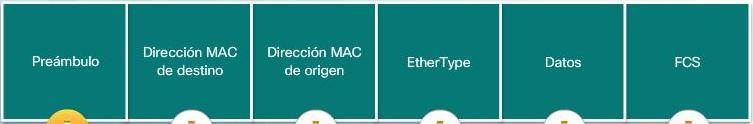
\includegraphics[width=0.9\textwidth]{./img/Campos-de-trama-de-Ethernet.jpg}
    \caption{Estructura de una trama Ethernet.}
    \label{fig:trama_ethernet}
\end{figure}


\subsection{¿Qué información permite determinar qué protocolo de capa superior está transportando una trama Ethernet?}

El campo \textbf{EtherType} de la trama Ethernet indica qué protocolo de capa superior se está transportando en el \textit{payload}. Es un valor de 2 bytes que el receptor lee para saber a qué módulo entregar los datos desencapsulados. Ejemplos:

\begin{itemize}
    \item \texttt{0x0800} $\rightarrow$ IPv4
    \item \texttt{0x86DD} $\rightarrow$ IPv6
    \item \texttt{0x0806} $\rightarrow$ ARP
    \item \texttt{0x8100} $\rightarrow$ VLAN (802.1Q)
\end{itemize}

\section{Ítem 2: Captura y análisis de tráfico con Wireshark}

\subsection{Seleccionar una trama Ethernet e identificar las direcciones MAC de origen y destino. ¿A qué dispositivos creen que corresponden?}

\subsection{Dentro de la misma trama, identificar el paquete IP. ¿Cuáles son las direcciones IP de origen y destino?}

\subsection{Comparar las direcciones MAC y las direcciones IP encontradas. ¿Representan lo mismo?}

\subsection{Observar el campo EtherType. ¿Qué protocolo está encapsulado dentro de la trama analizada?}

\section{Ítem 3: Transporte de información mediante TCP}

\subsection{¿Qué problema(s) resuelve TCP que no resuelve directamente Ethernet ni IP?}

\subsection{Investigar los campos más importantes de la metadata en un frame TCP. ¿Para qué sirve cada uno?}

\subsection{Explicar el Three-way y Four-way handshake en TCP.}

\subsection{Iniciar la conexión enviando un paquete, capturar el handshake y el paquete de datos. Analizar el paquete de datos, sus distintas partes y encontrar la carga útil del paquete usando Wireshark.}

\subsection{Finalizar la conexión y capturar el Four-way handshake.}

\subsection{¿Qué conclusión podemos sacar de que sea tan fácil ver un paquete que viaja a través de la red?}

\section{Ítem 4: Comunicación con un servidor remoto mediante PacketSender}

\subsection{Iniciar una conexión con el servidor y obtener respuestas para los comandos admitidos: hola, ping, tic y status.}

\subsection{Iniciar la conexión, enviar el comando correspondiente al grupo y documentar la respuesta del servidor.}

\end{document}
